Moderne Personenwagen sind recht genau, sie können das Gewicht einer
Person mit einem Fehler von $\varrho=0.1\text{kg}$ bestimmen.
Das Gewicht einer Person schwankt aber über den Tag ziemlich stark,
eine typische Mahlzeit ist ca 0.5kg schwer.
Selbst wenn jemand gar nichts tut, verliert er etwa 60g Gewicht pro
Stunde durch $\text{CO}_2$, welches er ausatmet.
Bleibende Gewichtsänderungen sind daher erst über längere Zeit erkennbar.
Mit Hilfe eines Kalman-Filters soll die Masse der Person möglichst genau
geschätzt werden.

\begin{teilaufgaben}
\item
Definieren Sie Zustandsvariablen, Zeitentwicklungsmatrix und Messmatrix
für diesen Kalmanfilter.
\item
Schätzen Sie die Fehlerkovarianzmatrizen ab.
\item 
Stellen Sie die Gleichungen des Kalman-Filters auf.
\item
Wenden Sie Ihren Kalman-Filter auf die Messdaten im File \texttt{m.csv} an.
Verwenden Sie dazu entweder ein Programm zum Beispiel in Matlab, Octave oder
irgend einer anderen Programmiersprache, oder verwenden Sie ein Spreadsheet
zur Durchführung der Rechnung.
\item
Da $\varphi_k$, $H_k$ und die Kovarianzmatrizen nicht von $k$ abhängen,
stellen sich für $K_k$ und $P_k$ stabile Werte einstellen.
Welche Werte hat ihre Simulation gefunden?
\item
Wie genau kann der Filter das tatsächliche Gewicht feststellen?
Verwenden Sie dazu, dass die Masse ursprünglich während der ersten
100 Datenpunkte konstant den Wert 70 hatte, und während der letzten
100 Datenpunkte konstant den Wert 75.
Dazwischen nahm die Masse linear zu.
\item
Die Performance des Kalman-Filters ist etwas enttäuschend, was aber
vor allem auf den relativ grossen Systemfehler zurückzuführen
ist\footnote{Die Datenqualität könnte deutlich verbessert werden, wenn
die Person sich zum Beispiel immer am Morgen nach dem Aufstehen wägen
würde.}.
Eine leichte Verbesserung kann erreicht werden, indem man auch die
täglichen Schwankungen zum Messfehler zählt, also $\varrho$ vergrössert
und $\sigma$ verkleinert. 
\end{teilaufgaben}

\begin{loesung}
\begin{teilaufgaben}
\item
Die Zustandsvariable, die uns interessiert, ist die Masse $m$ der Person.
Der Zustandsvektor hat daher nur eine Komponenten:
\[
x_k = \begin{pmatrix}m_k\end{pmatrix}.
\]
Da sich das Gewicht nur sehr langsam ändert, können wir ein Modell verwenden,
welches von einer konstanten Masse ausgeht.
Die Entwicklungsgleichung wird daher
\[
x_{k+}
=
\begin{pmatrix}m_{k+1}\end{pmatrix}
=
\underbrace{\begin{pmatrix}1\end{pmatrix}}_{\displaystyle=\varphi_k}
\begin{pmatrix}m_k\end{pmatrix}
=
\varphi_kx_k.
\]
Die Waage misst die einzige Zustandsvariable, die Matrix $H$ ist
daher die Einheitsmatrix 
\[
H_k = \begin{pmatrix}1\end{pmatrix}
\]
\item
Der Messfehler ist bekannt, die Messfehlerkovarianzmatrix ist daher
\[
R_k
=
\begin{pmatrix} \varrho^2\end{pmatrix}
=
\begin{pmatrix} 0.01\,\text{kg}^2\end{pmatrix}.
\]
Die Systemfehlerkovarianz muss die Veränderungen der Masse über den Tag
wiedergeben, die im Systemmodell keinen Eingang gefunden haben.
Gemäss Beschreibung in der Aufgabenstellung wird die gleichmässige
Abnahme der Masse durch den Metabolismus unterbrochen von Sprüngen.
Insgesamt kann man daher von einer in einem Interval um die mittlere
Masse gleichverteilten Masse ausgehen.
Wir schätzen die Intervalbreite auf etwa 0.6\,kg.
Die Varianz einer Gleichverteilung mit 0.6\,kg Intervalbreite ist
\[
\sigma^2 = \frac{0.6^2}{12}\text{kg}^2 = 0.03\,\text{kg}^2.
\]
\item
Die Kalman-Filter-Formeln sind in diesem Beispiel besonders einfach,
weil alle Matrizen nur eine Komponente haben.
Die Messfehlerkovarianzmatrix ist auch nur eine einzige Zahl, wir
schreiben $P_k=\begin{pmatrix}p_k^2\end{pmatrix}$.
Die Kalman-Filter-Formeln sind:
\begin{align*}
\hat m_{k|k-1}&=\hat m_k
&
\hat m_k&=(1-K_k)\hat m_{k|k-1} + K_kz_k
=
\hat m_{k|k-1} + K(z_k-\hat m_{k|k-1})
\\
\hat p_{k|k-1}^2&=\hat p_{k-1}^2 + \sigma^2
&
\hat p_k^2&=(1-K)^2\hat p_{k|k-1}^2+K^2\varrho^2
\\
&&
K_k&=\hat p_{k|k-1}(\hat p_{k|k-1}^2+\varrho^2)^{-1}
\end{align*}
Die Formeln links beschreiben den Vorhersageschritt, die Formeln rechts
dagegen den Korrekturschritt.
Fassen wir die Formeln zusammen, erhalten wir
\begin{align*}
K_k
&=
\frac{\hat p_{k-1}^2 + \sigma^2}{\hat p_{k-1}^2+\sigma^2+\varrho^2}
\\
\hat m_k
&=
\hat m_{k-1} + K_k(z_k - \hat m_{k-1})
\\
\hat p_k^2
&=
(1-K_k)(\hat p_{k-1}^2+\sigma^2)
\end{align*}
Dabei haben wir in der lezten Formel die Vereinfachung verwendet, die in
Satz~8.2 im Skript dargestellt ist.
\item
Eine mögliche Lösung ist 
\verbatimainput{kalman.m}
\item
Die Resultate des Filter sind in Abbildung~\ref{90000007:filter1}
dargestellt.
Die gesuchten Werte für $p_k^2$  und $K_k$ sind in der Graphik dargestellt.
\item
In den graphischen Darstellungen wird auch die mittlere quadratische
Abweichung dargestellt.
Für den ursprünglichen Filter ist erreichte Schätzfehler etwa 150\,g,
die Rohdaten haben jedoch eine Standardabweichung von den Modelldaten
von 200\,g.
\item
Derwendet man $\sigma^2=0.04$ und $\varrho^2 = 0.001$ für den Filter,
erhält man die Resultate in Abbildung~\ref{90000007:filter2}.
Man erkennt, dass sich so der Schätzfehler auf etwa 120\,g reduzieren
lässt.
\end{teilaufgaben}
\begin{figure}
\centering
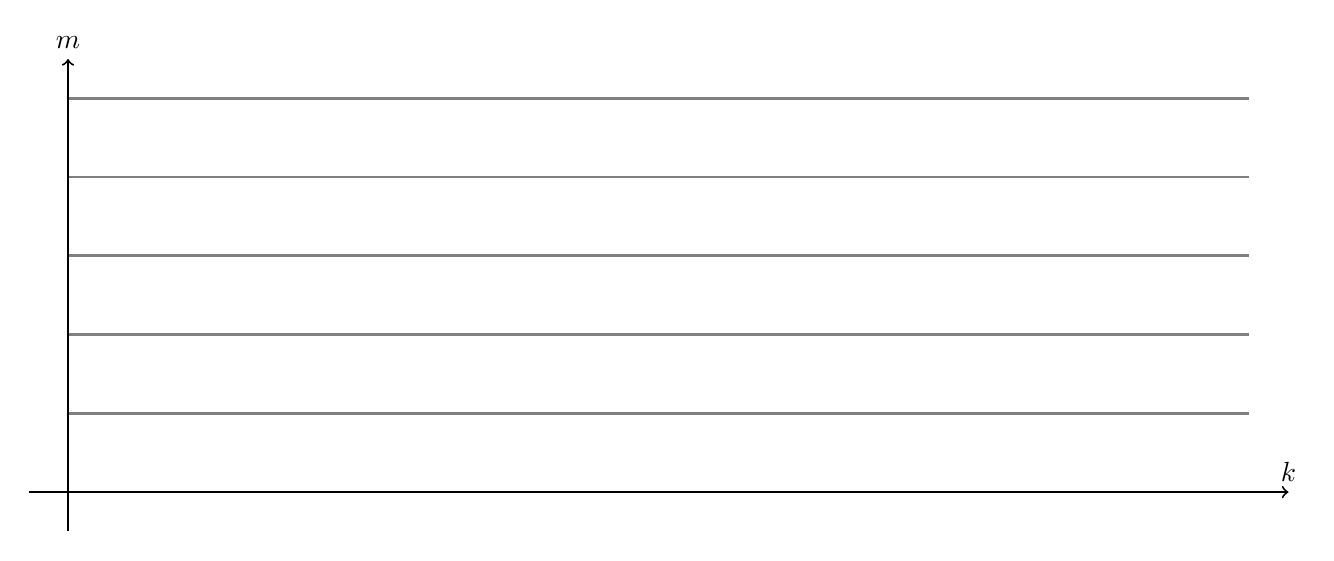
\begin{tikzpicture}[scale=1]
\foreach \y in {0,1,...,5}{
	\draw[color=gray,line width=1pt] (0,{\y})--(15,{\y});
}
\draw[->,line width=0.7pt] (-0.5,0)--(15.5,0) coordinate[label={$k$}];
\draw[->,line width=0.7pt] (0,-0.5)--(0,5.5) coordinate[label={$m$}];
\ainput{gewicht.tex}
\end{tikzpicture}
\caption{Filterung durch den Kalman-Filter.
Nur die ausgeprägtesten Spitzen vermag der Filter zu entfernen.
\label{90000007:filter1}
}
\end{figure}
\begin{figure}
\centering
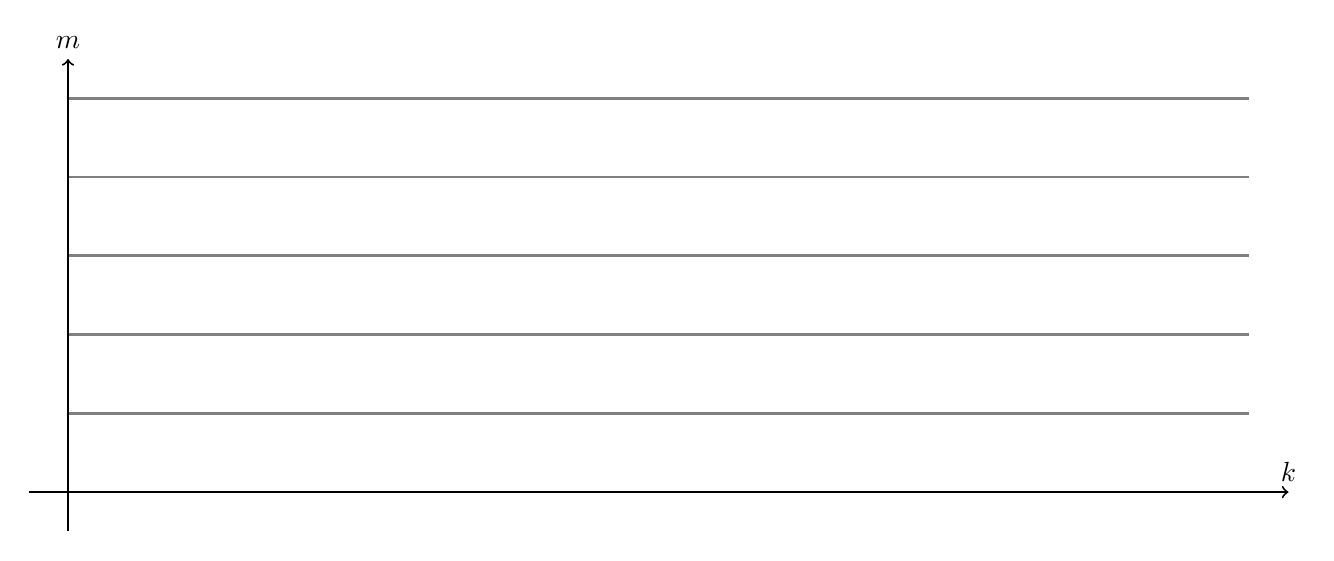
\begin{tikzpicture}[scale=1]
\foreach \y in {0,1,...,5}{
	\draw[color=gray,line width=1pt] (0,{\y})--(15,{\y});
}
\draw[->,line width=0.7pt] (-0.5,0)--(15.5,0) coordinate[label={$k$}];
\draw[->,line width=0.7pt] (0,-0.5)--(0,5.5) coordinate[label={$m$}];
\ainput{gewicht2.tex}
\end{tikzpicture}
\caption{Resultate der Filterung unter der Annahme, dass die Schwankungen
sich vollständig im Messfehler äussern.
\label{90000007:filter2}
}
\end{figure}
\end{loesung}

\begin{diskussion}
Angesichts der relativ grossen, nicht modellierbaren Schwankungen und
der offensichtlichen Unmöglichkeit, diese auch mit einem optimalen
Filter wieder zu entfernen, wird klar, dass eine Personenwaage mit einer
grösseren Genauigkeit als 100\,g nicht sinnvoll sein kann.
\end{diskussion}



